\chapter{動作検証}
\thispagestyle{myheadings}
本アプリの動作検証は特定の時空間に進入時のみセンシングできているか,プラットフォームとして複数のユースケースを想定して適切にセンシングできているかの2つを行う.
本アプリは時空間フェンシングを基盤にしている.そのため,時空間フェンシングの適切な動作が必須になる.
その中でも\ref{myApp_STF}章で述べた任意の多角形に対応したマージンとジオフェンシングが適切に動作するか確認する.
任意の多角形に対して適切な動作が確認できれば,単純な矩形にも対応できているとする.

本アプリはプラットフォームとして様々なクラウドセンシングに対応する必要がある.
そのため本アプリの動作検証として複数のユースケースを想定して期待された動作が確認できるかを確認する.
本論の動作検証では,天候毎の移動速度推定とコミュニケーション推定に利用されたと仮定し適切に動作するか,集められたセンサデータから目的を達成できたかを確認する.

\section{時空間フェンシングの動作検証}
% 目的,環境,結果,考察
ジオフェンスが任意の多角形の時,マージンを含め適切に動作しているか検証した.
動作検証の設定と評価項目を図\ref{fig:ex_margin_1}に示す.
図\ref{fig:ex_margin_1}左部のように多角形のジオフェンスを設け,ジオフェンスを通過するように移動する(図\ref{fig:ex_margin_1}橙色矢印).
評価項目を図\ref{fig:ex_margin_1}右部に記す.
まず,ジオフェンスに進入する可能性が高い協力者に通知を発行しているか確認する.
ジオフェンスに進入する可能性が高い協力者は\ref{myApp_notify}章で述べた通りである.
\ref{myApp_STF}章で述べた通り,協力者につけた内外判定を持つ点が1つ以上ジオフェンスの内側にある時,拡大したジオフェンスに進入したと判定し通知を発行する.
次に,確実にジオフェンシングの内側にいる時にセンシングを開始するか確認する.
適切に動作している場合,協力者につけた内外判定を持つ点全てがジオフェンスに進入した時,確実にジオフェンスの内側にいると判定しセンシングを開始する.
最後に,確実にジオフェンスから退出している場合センシングが終了するか確認する.
適切に動作している場合,協力者につけた内外判定を持つ点全てがジオフェンスから退出した時,確実にジオフェンスの外側にいると判定しセンシングが終了する.

\begin{figure}[tbh]
    \centering
    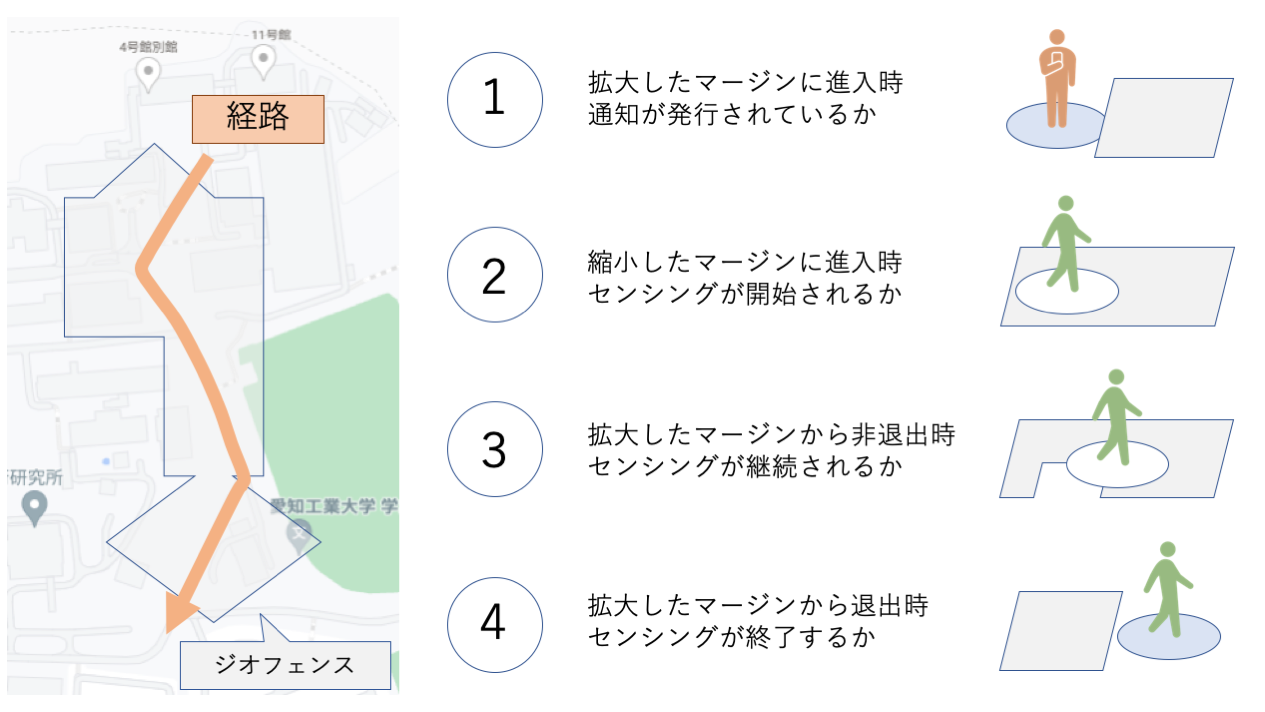
\includegraphics[width=16cm]{img_ex_margin_1.png}
    \caption{ジオフェンシングの動作検証}
    \label{fig:ex_margin_1}
\end{figure}

動作検証の結果は図\ref{fig:ex_margin_2}に示す.
まず,拡大したジオフェンスに進入した時に通知の発行を確認した.
次に,縮小したジオフェンスに進入した時にセンシングが開始するのを確認した.
最後に,拡大したジオフェンスから退出した時にセンシングが終了するのを確認した.
以上から,適切な動作が確認できたと言える.

\begin{figure}[tbh]
    \centering
    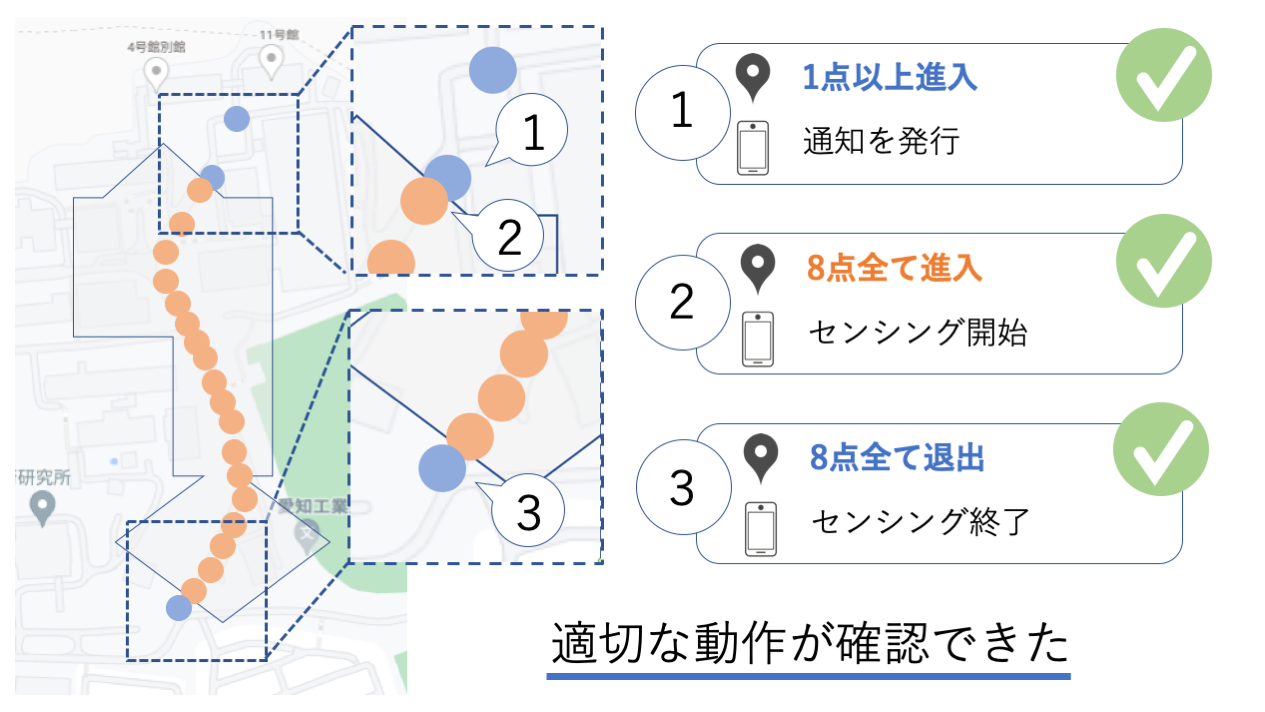
\includegraphics[width=16cm]{img_ex_margin_2.png}
    \caption{ジオフェンシングの動作検証の結果}
    \label{fig:ex_margin_2}
\end{figure}
% (屋内でもやる)

\section{ユースケースを想定した動作検証}
天候によって所要時間が変化する地図アプリを作成したい人がいたと仮定する.
また,その人は依頼者として天候毎の移動速度のデータ収集に本システムを利用し,本アプリはその依頼者の作成したセンシングプロジェクトをダウンロードしたとする.
依頼者は時空間を歩行者の多い8時30分から16時50分の愛知工業大学と設定し,使用するセンサを線形加速度とGPSとした(図\ref{fig:ex_case_1}).

\begin{figure}[tbh]
    \centering
    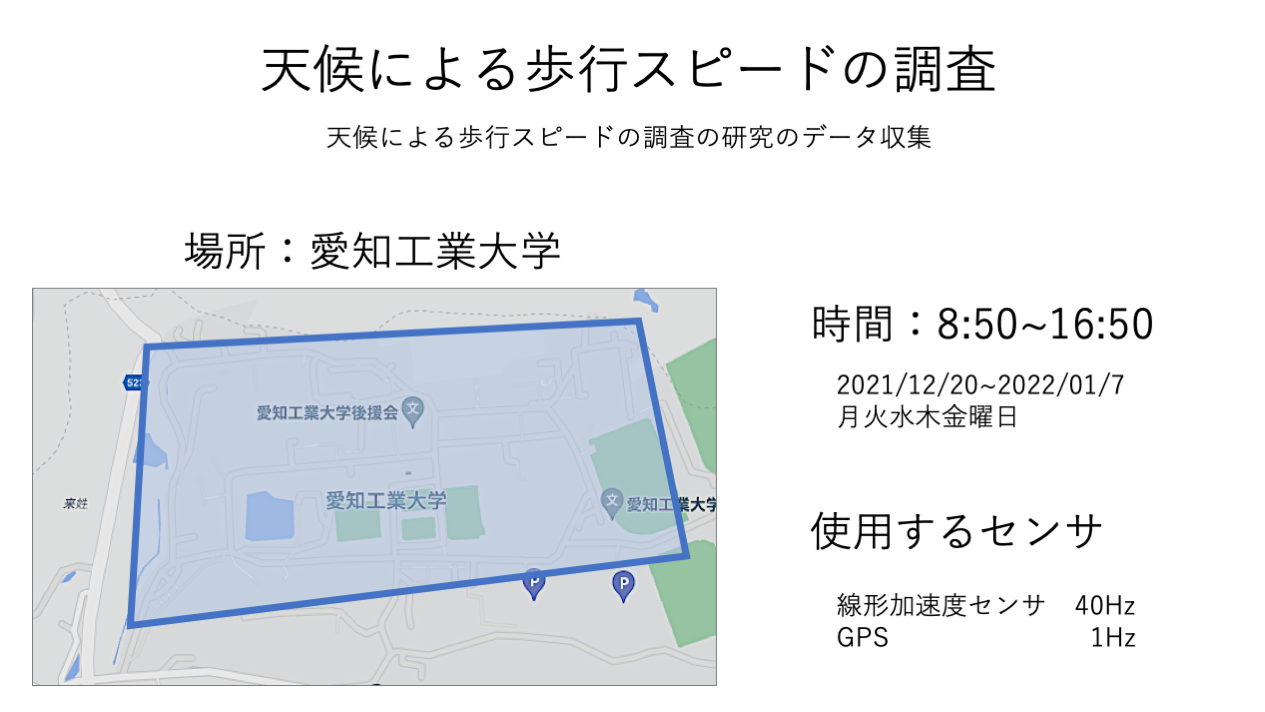
\includegraphics[width=16cm]{img_ex_case_1.png}
    \caption{天候による歩行スピードの調査の実験設定}
    \label{fig:ex_case_1}
\end{figure}

線形加速度のデータは歩行推定に利用し,GPSは移動速度推定に利用する.
また,その時の天候はセンシングされた時間とGPSから取得する.
本アプリは依頼者の作成したセンシングプロジェクトに基づいてセンシングした.
本アプリによっていくつかの線形加速度センサとGPSのセンサデータが得られた.
まず,依頼者はGPSログと時間データから移動速度を求めた.
次に,依頼者は線形加速度から歩数推定と歩幅推定を行なった.
結果,いくつかのセンサデータからは適切だと思える歩数や歩幅が求められた.
しかし,いくつかのセンサデータからは明らかに異常な歩数や歩幅が推定された.

これは,協力者の端末の携帯方法に違いがあったと考える.
今回使用した歩数推定アルゴリズムは腰周辺に端末が携帯されている場合のアルゴリズムのため,サイドポケットや鞄に端末でセンシングした場合は使用できない.
そのため協力者の端末の携帯方法を固定するか,協力者の端末の携帯方法の推定をする必要がある.
しかし,センシング依頼画面を通して協力者に端末の携帯方法を伝えられるが,実際に協力者がその携帯方法をするとは限らない.
このようにセンシング方法に条件がある場合は,協力者の端末の携帯方法を推定する必要があると考える.

次に,研究室の管理者が,研究室内でどれだけコミュニケーションが取られているか測定しようとしたと仮定する.
研究室の管理者は依頼者として研究室内におけるコミュニケーション推定に本システムを利用し,本アプリはその依頼者の作成したセンシングプロジェクトをダウンロードしたとする.
時空間を8時30分から21時の研究室と設定し,使用するセンサを音センサと加速度センサとした(図\ref{fig:ex_case_2}).

\begin{figure}[tbh]
    \centering
    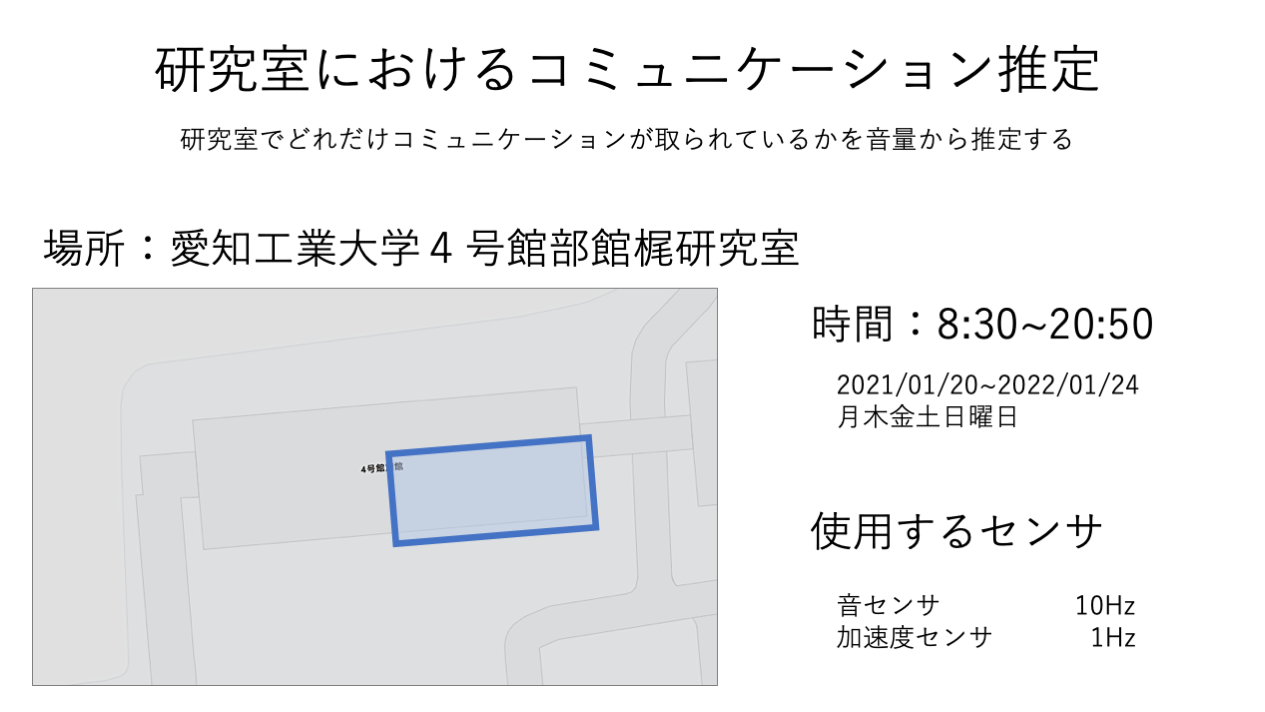
\includegraphics[width=16cm]{img_ex_case_2.png}
    \caption{研究室におけるコミュニケーション推定の実験設定}
    \label{fig:ex_case_2}
\end{figure}

依頼者は,加速度センサとから端末の状態を推定した.
端末が協力者のポケットに中にある場合や協力者が端末を使用している場合,布の擦れる音やタップ音などがセンシングされてしまう.
依頼者端末が机等の安定した場所にあるか推定するため,加速度センサを使用した.
依頼者は端末が机等の安定した場所にある時の音センサのデータを抽出し,研究室内で発生した音からコミュニケーションを推定した(図\ref{fig:ex_case_2_audio}).

\begin{figure}[tbh]
    \centering
    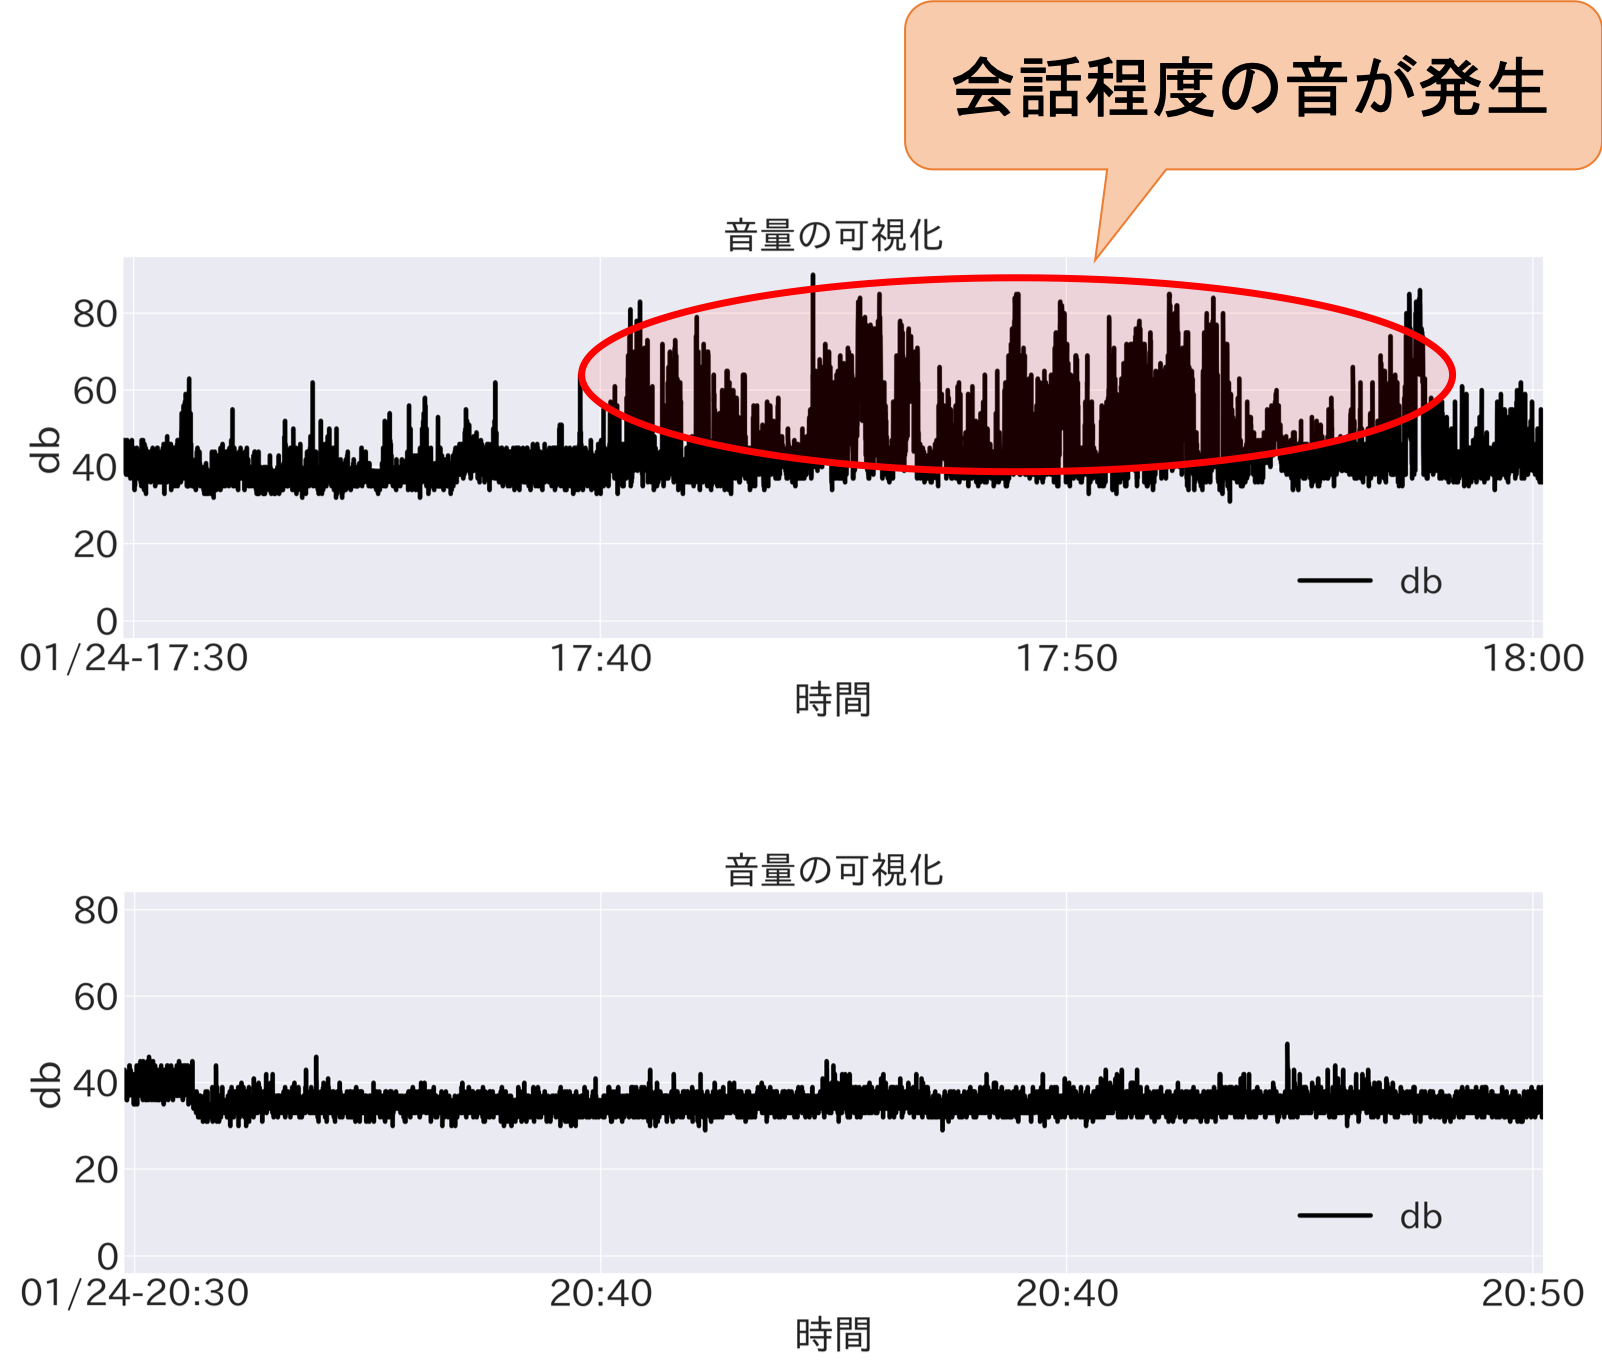
\includegraphics[width=16cm]{img_ex_case_2_audio.png}
    \caption{研究室内でのコミュニケーション推定}
    \label{fig:ex_case_2_audio}
\end{figure}

騒音の大きさの目安\ref{db}を参考に抽出した音センサのデータから会話程度の音を発見した.
結果,集めたセンサデータから時間帯ごとの賑やかさが推定できた.
また,研究室で管理している滞在者情報と合わせて研究室に所属する生徒単位の仲良し度推定に応用ができると考える.


% Local Variables: 
% mode: japanese-LaTeX
% TeX-master: "root"
% End: 
